\chapter{Mathematical modelling}

Mathematical models can describe different kinds of dynamic systems, and thus can be used in prediction, analysis and other tasks. An ideal model in our case, can represent reasonable interactions or effects between immune cells and cytokines and reproduce features and characteristics that were observed in experimental data.

Proposed models for the regeneration process were in the form of non-linear ordinary differential equations (ODE). The only independent variable is post-lesion time $t$. The equations consist of four derivatives of dependent variables (number of cells, mRNA expression of cytokines) with respect to $t$. The equations were mostly an interpretation of the proposed interaction maps, with terms correspond to interaction paths.


\section{Observed data}

Our models were built based on the existing experimental findings from Tsarouchas et al. \cite{ref:Tsarouchas}. The available measurement data included the numbers of three kinds of cells (neutrophil $N$, macrophage $\Phi$ and microglia) and the relative mRNA expression of four kinds of cytokines (il-1$\beta$, tnf-$\alpha$, tgf-$\beta$1a and tgf-$\beta$3). As proposed by Tsarouchas et al., neutrophil and macrophage play essential roles in controlling the il-1$\beta$ and tnf-$\alpha$ mediated inflammation. Our initial models focused on the changes of four dependent variables $N$, $\Phi $, $\beta$ (for il-1$\beta$) and $\alpha$ (for tnf-$\alpha$) that are most important and determinative in the regeneration. $N$ and $\Phi$ is of the unit `number of cells', $\beta$ and $\alpha$ is recorded as `relative mRNA expression' (compared to the value at the initial time point, i.e. 0 hpl) and considered unitless.

It was noted that the variance of the measured data is relatively high. The summary statistic was the mean of measurement data at each time point, assuming that measured data was Gaussian-like distributed. To validate this, the distribution of the measured data points was plotted. The result was that at most time points the measurement values are Gaussian-distributed, although some distributions were skewed. One abnormal distribution was observed at time point 120 hpl for macrophage where there are two concentrations. Despite this, the mean value could summarise most data and thus was still used as the target summary data. The mean value at each time point is shown in Figure \ref{fig:obs_data}, which is our target trajectories for the models to fit.

\begin{figure}
    \begin{center}
        \resizebox{1.0\hsize}{!}{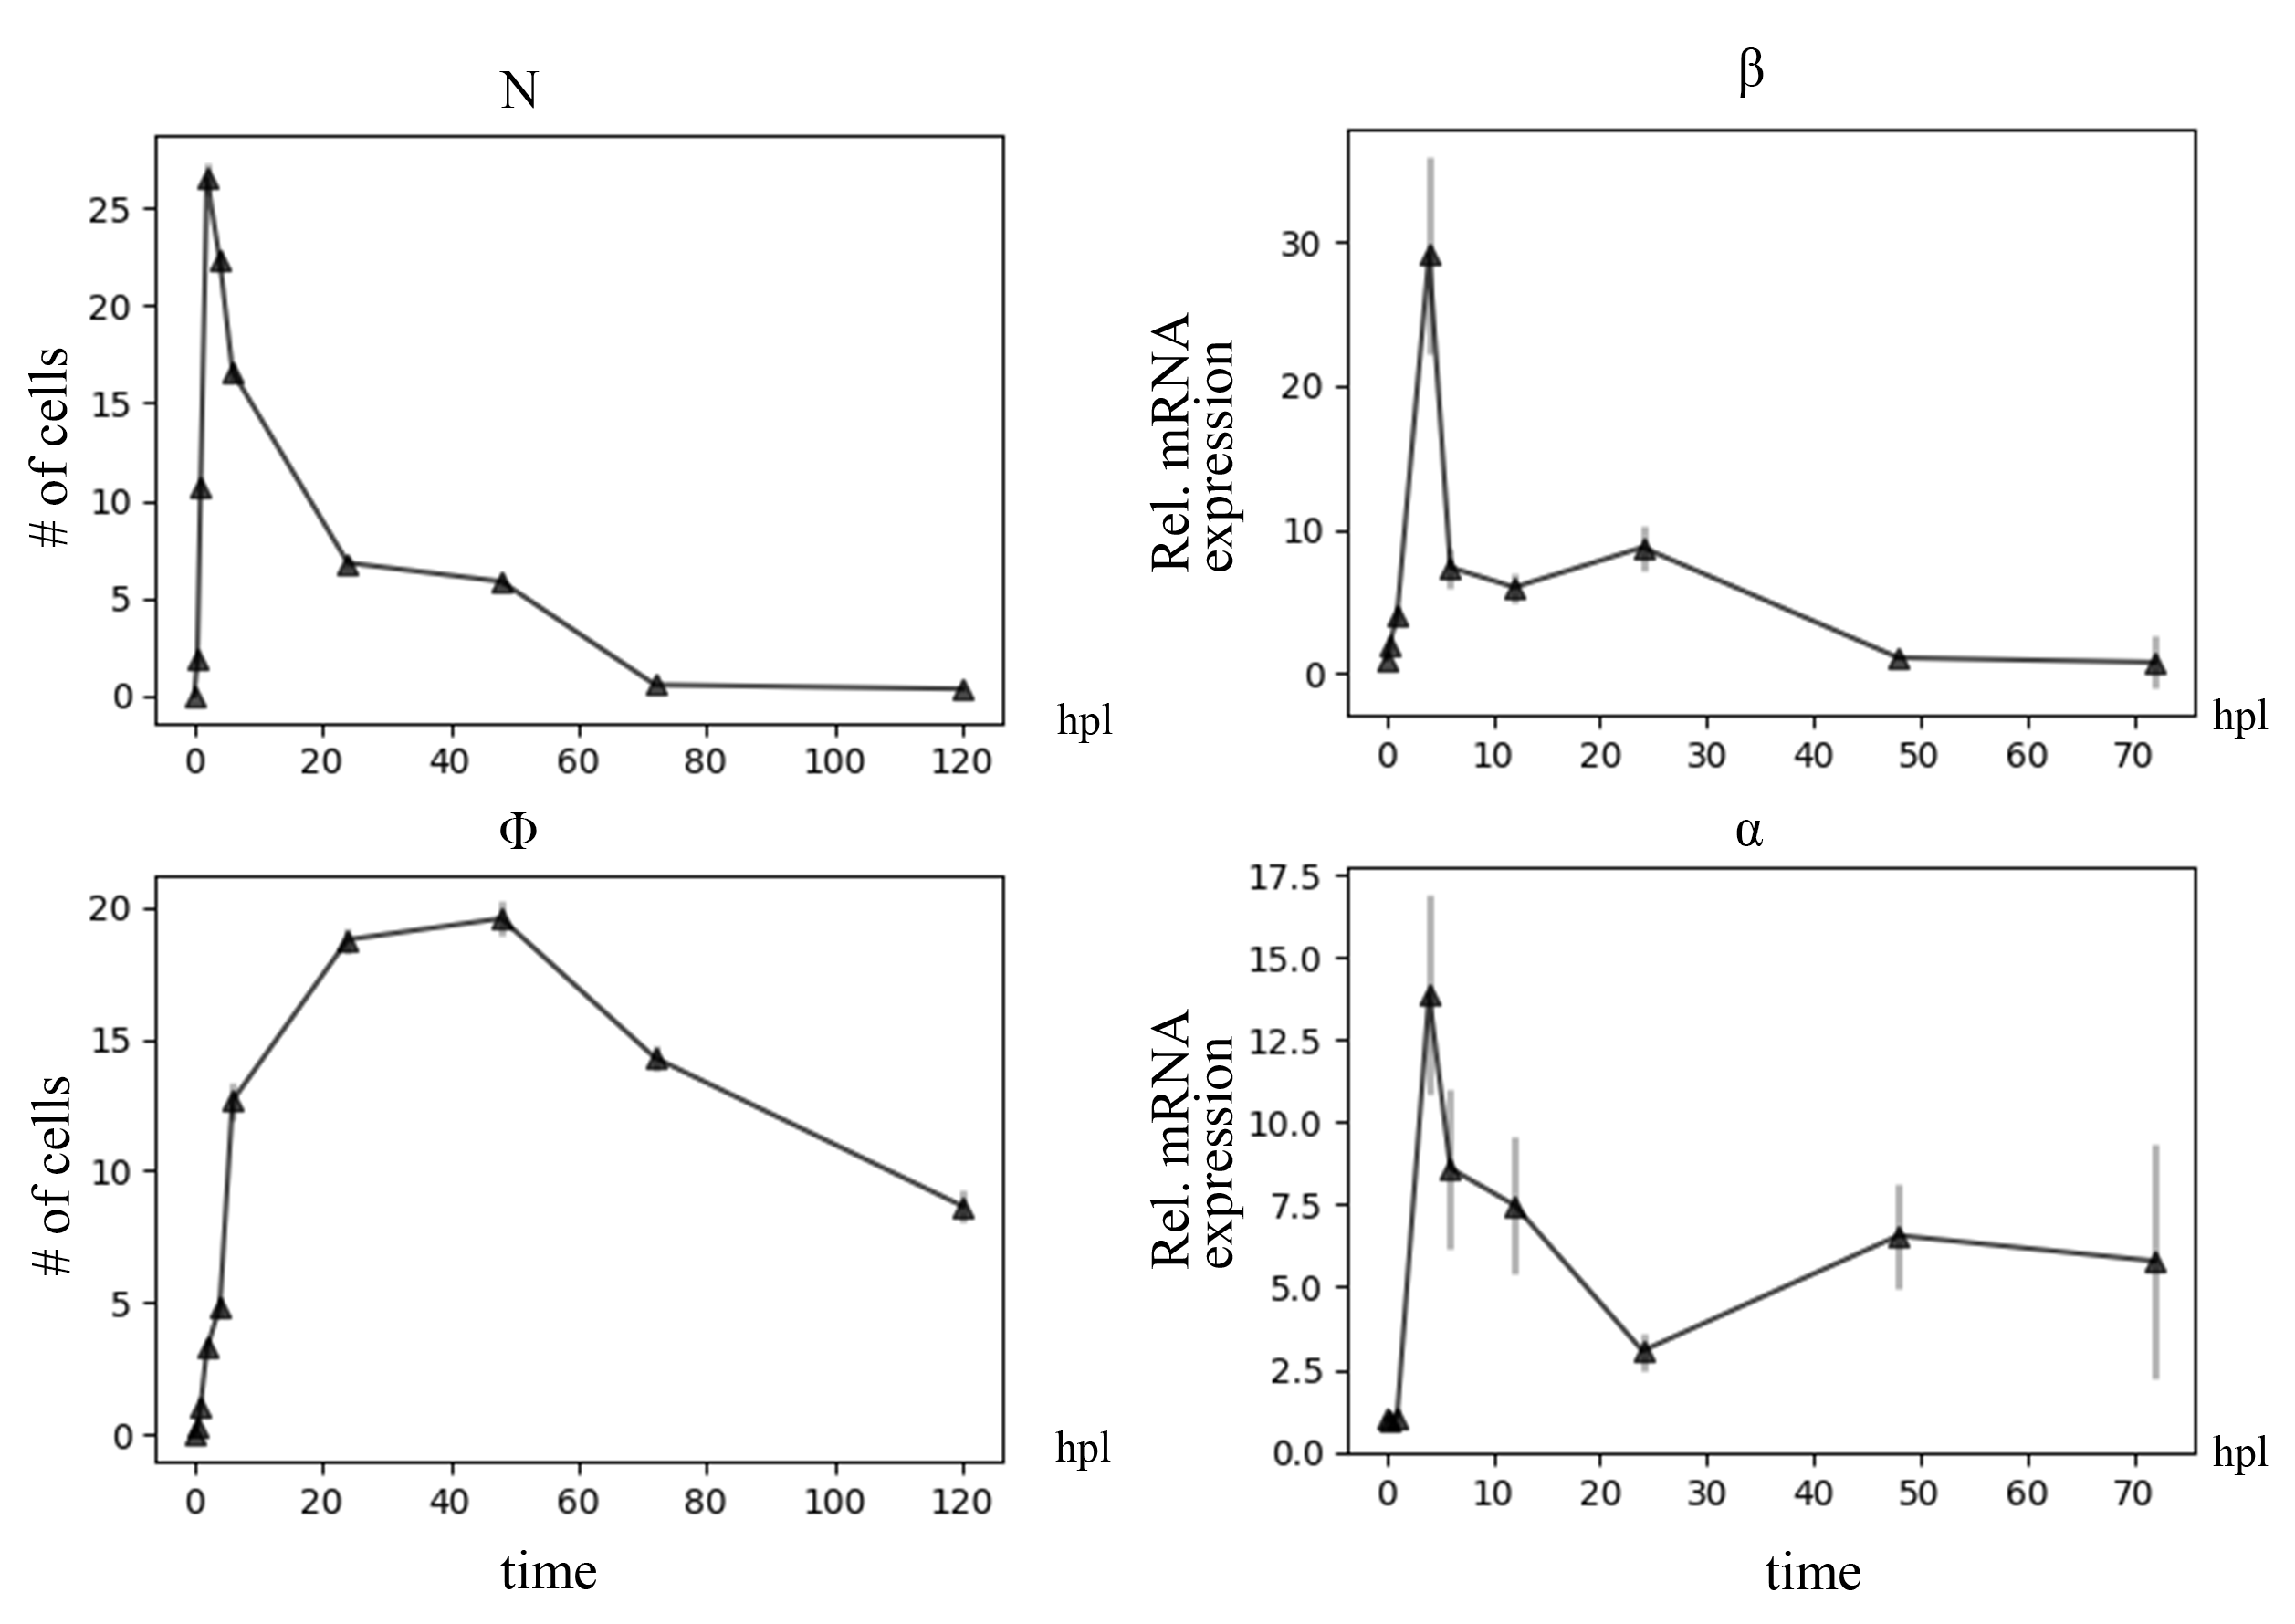
\includegraphics{fig/observed.png}}
    \end{center}

    \caption[Mean of the observed data]%
    {Mean of the observed data for neutrophil ($N$), macrophage ($\Phi$), il-1$\beta$ and tnf-$\alpha$, from experiment results of \cite{ref:Tsarouchas}. Error bars indicate standard error of mean (SEM). For $N$ and $\Phi$ the SEM is relatively small}
    \label{fig:obs_data}

\end{figure}

\section{Hypotheses and models}

Five models in total are proposed according to different hypotheses. At first, our tests and implementations of ABC SMC for parameter estimations used only the basic model for developing propose. After the parameter inference framework was built and tested, more models were proposed in order to calibrate and improve the basic model such that the observed regeneration process can be better represented.

All these models assumed that the involved interactions are within two kinds of cells (neutrophil and macrophage) and two kinds of cytokines (il-1$\beta$ and tnf-$\alpha$), and used the data presented in Figure \ref{fig:obs_data} for the inference task. Interactions or influences from other cells or cytokines are not considered as there might not be corresponding data available. If such data or experimental findings are available in the future, we can consider them by then as long as these interactions are indeed necessary for our model.

\subsection{Basic model}

A preliminary model (Eqn. \ref{eq:model1}) was proposed according to \cite{ref:Tsarouchas} and then mainly used to build and test the code of inference framework. An interaction map of the model is shown in Figure \ref{fig:m1}. This model is a simplification of the process described in \cite{ref:Tsarouchas} (Figure \ref{fig:map}) with some minor interactions ignored. This model included 12 parameters, all of which should be positive real numbers. A description of these parameters can be found in Table \ref{table:m1}.

\begin{figure}
    \begin{center}
        \resizebox{0.4\hsize}{!}{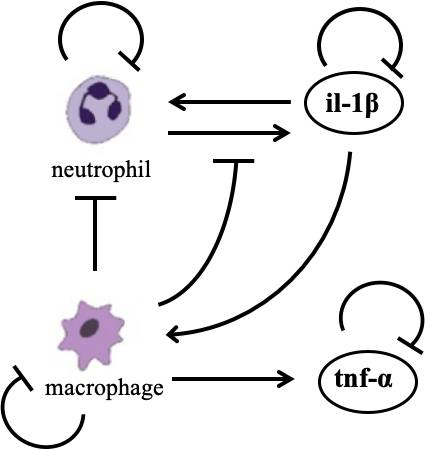
\includegraphics{fig/model1.png}}
    \end{center}

    \caption[Interactions modelled in the basic model]%
    {Interactions modelled in the basic model (model 1) based on Tsarouchas et al.\cite{ref:Tsarouchas}. Lines ended with arrow represent promoting effect, lines ended with T-connectors represent inhibition}
    \label{fig:m1}

\end{figure}

\begin{align}
    \label{eq:model1}
    \begin{split}
        &\frac{\mathrm{d} N}{\mathrm{d} t}=\lambda_N+\kappa_{N\beta}\beta-\mu_NN-\nu_{N\Phi}N\Phi\\
        &\frac{\mathrm{d} \Phi}{\mathrm{d} t}=\lambda_\Phi+\kappa_{\Phi\beta}\beta-\mu_\Phi\Phi\\
        &\frac{\mathrm{d} \beta}{\mathrm{d} t}=\frac{s_{\beta N}N}{1+i_{\beta\Phi}\Phi}-\mu_\beta\beta\\
        &\frac{\mathrm{d} \alpha}{\mathrm{d} t}=s_{\alpha\Phi}\Phi-\mu_\alpha\alpha
    \end{split}
\end{align}

It was assumed that there are negative feedbacks the cells and cytokines, i.e. overcrowding inhibits the increasing rates. As sources, macrophage produces tnf-$\alpha$ and neutrophil produces il-1$\beta$; however, macrophage was assumed to have a negative effect on the il-1$\beta$, term $1+i_{\beta\Phi}\Phi$ in Eqn. \ref{eq:model1} was used to represent this. Despite the self-driven increase of immune cells, il-1$\beta$ was assumed to promote the increase of both cells. Neutrophil was also assumed to be inhibited by the total immune cells presented in the lesion site, the term $\nu_{N\Phi}N\Phi$ was used to denote this.

\begin{table}[t]
    \centering
    \begin{tabular}{|c c c|}
        \hline
        Parameter            & Definition                                       & Units                    \\ [0.5ex]
        \hline\hline
        $\lambda_N$          & Self-increase rate of neutrophil                 & $cell/h$                 \\
        $\kappa_{N\beta}$    & Promoting effect coefficient by il-1$\beta$      & $cell/h$                 \\
        $\mu_N$              & Coefficient of negative feedback of $N$          & $h^{-1}$                 \\
        $\nu_{N\Phi}$        & Coefficient of inhibition of both $N$ and $\Phi$ & $cell^{-1}\cdotp h^{-1}$ \\
        \hline
        $\lambda_\Phi$       & Self-increase rate of macrophage                 & $cell/h$                 \\
        $\kappa_{\Phi\beta}$ & Promoting effect coefficient by il-1$\beta$      & $cell/h$                 \\
        $\mu_\Phi$           & Coefficient of negative feedback of $\Phi$       & $h^{-1}$                 \\
        \hline
        $s_{\beta N}$        & Production rate from $N$                         & $cell^{-1}\cdotp h^{-1}$ \\
        $i_{\beta\Phi}$      & Coefficient of inhibition to the production      & $cell^{-1}$              \\
        $\mu_\beta$          & Coefficient of negative feedback of $\beta$      & $h^{-1}$                 \\
        \hline
        $s_{\alpha\Phi}$     & Production rate from $\Phi$                      & $cell^{-1}\cdotp h^{-1}$ \\
        $\mu_\alpha$         & Coefficient of negative feedback of $\alpha$     & $h^{-1}$                 \\
        \hline
    \end{tabular}
    \caption{Parameters introduced in the basic model (model 1) [REMOVE unit]}
    \label{table:m1}
\end{table}

\subsection{Alternative models}

\paragraph{Model 2 and model 3}

As the observed data indicated, this dynamic system has a steady-state where after a long time ($\geq 120$ hpl), the inflammation is resolved, and immune cells should not be present at the injury site any more. Regarding this, the parameter for self-increase rate for the macrophage and neutrophil, i.e. $\lambda_\Phi$ and $\lambda_N$  cannot be constant. An exponentially decaying $\lambda$ term is introduced in the new model (model 2, Eqn. \ref{eq:model2}). Also, the inhibition of il-1$\beta$ production, i.e. the term $i_{\beta\Phi}\Phi$ is considered to be ignored for a more simple model, in which case the relative expression of il-1$\beta$ is only affected by the number of neutrophils and the negative feedback from itself. This case corresponds to model 3, written as Eqn. \ref{eq:model3}.

Model 2 and model 3 introduced one extra parameter $a$ and removed $\lambda_\Phi$, which is a coefficient in the exponentially decaying $\lambda_N$, determining the decay speed, with the unit $h^{-1}$.

\begin{align}
    \label{eq:model2}
    \begin{split}
        &\frac{\mathrm{d} N}{\mathrm{d} t}=\lambda_Ne^{-at}+\kappa_{N\beta}\beta-\mu_NN-\nu_{N\Phi}N\Phi\\
        &\frac{\mathrm{d} \Phi}{\mathrm{d} t}=\kappa_{\Phi\beta}\beta-\mu_\Phi\Phi\\
        &\frac{\mathrm{d} \beta}{\mathrm{d} t}=\frac{s_{\beta N}N}{1+i_{\beta\Phi}\Phi}-\mu_\beta\beta\\
        &\frac{\mathrm{d} \alpha}{\mathrm{d} t}=s_{\alpha\Phi}\Phi-\mu_\alpha\alpha
    \end{split}
\end{align}

\begin{align}
    \label{eq:model3}
    \begin{split}
        &\frac{\mathrm{d} N}{\mathrm{d} t}=\lambda_Ne^{-at}+\kappa_{N\beta}\beta-\mu_NN-\nu_{N\Phi}N\Phi\\
        &\frac{\mathrm{d} \Phi}{\mathrm{d} t}=\kappa_{\Phi\beta}\beta-\mu_\Phi\Phi\\
        &\frac{\mathrm{d} \beta}{\mathrm{d} t}=s_{\beta N}N-\mu_\beta\beta\\
        &\frac{\mathrm{d} \alpha}{\mathrm{d} t}=s_{\alpha\Phi}\Phi-\mu_\alpha\alpha
    \end{split}
\end{align}

Model 3 can be regarded as a simplification of model 2, as it can be treated as model 2 with parameter $i_{\beta\Phi}=0$. Among the proposed three models, model 1 is a naive one that was proposed at the very first time and used as an ODE `template' to build and test our parameter inference framework. As the implementation was successful, model 2 and 3 was proposed, as we were trying to calibrate some terms and find better models. After fitting, model 2 is supposed to be better than model 1 as it corrects the problem that appears at the final time points (which were related to the steady states of immune cells). Model 3 made a small simplification based on model 2, and thus it was theoretically less `general' than model 2.

\paragraph{Model 4 and model 5}

After the first model selection experiment among the exiting three models, it was found that any of the models did not recover some significant features presented in the observed data. To resolve this, attempts were tried to introduce additional reasonable interactions within the dynamic system, considering the biological and mathematical context. Extra promoting effect to the expression of tnf-$\alpha$ was considered, by either adding a phenomenological term $d_{\beta\alpha}\beta$ (which means the same effect as directly promoting but the underlying mechanism is unclear), or adding a term $f_{\beta\alpha}$ that represents a promoting effect to the production process of tnf-$\alpha$, namely model 4 (Eqn. \ref{eq:model4}) and model 5 (Eqn. \ref{eq:model5}).

\begin{align}
    \label{eq:model4}
    \begin{split}
        &\frac{\mathrm{d} N}{\mathrm{d} t}=\lambda_Ne^{-at}+\kappa_{N\beta}\beta-\mu_NN-\nu_{N\Phi}N\Phi\\
        &\frac{\mathrm{d} \Phi}{\mathrm{d} t}=\kappa_{\Phi\beta}\beta-\mu_\Phi\Phi\\
        &\frac{\mathrm{d} \beta}{\mathrm{d} t}=s_{\beta N}N-\mu_\beta\beta\\
        &\frac{\mathrm{d} \alpha}{\mathrm{d} t}=s_{\alpha\Phi}\Phi-\mu_\alpha\alpha+d_{\beta\alpha}\beta
    \end{split}
\end{align}

\begin{align}
    \label{eq:model5}
    \begin{split}
        &\frac{\mathrm{d} N}{\mathrm{d} t}=\lambda_Ne^{-at}+\kappa_{N\beta}\beta-\mu_NN-\nu_{N\Phi}N\Phi\\
        &\frac{\mathrm{d} \Phi}{\mathrm{d} t}=\kappa_{\Phi\beta}\beta-\mu_\Phi\Phi\\
        &\frac{\mathrm{d} \beta}{\mathrm{d} t}=s_{\beta N}N-\mu_\beta\beta\\
        &\frac{\mathrm{d} \alpha}{\mathrm{d} t}=(s_{\alpha\Phi}+f_{\beta\alpha}\beta)\Phi-\mu_\alpha\alpha
    \end{split}
\end{align}

\begin{table}[h!]
    \centering
    \begin{tabular}{|c c c|}
        \hline
        Parameter         & Definition                                                     & Units                    \\ [0.5ex]
        \hline\hline
        $d_{\beta\alpha}$ & Coefficient of promoting effect from $\beta$                   & $h^{-1}$                 \\
        \hline
        $f_{\beta\alpha}$ & Coefficient of promoting the production of $\alpha$ by $\beta$ & $cell^{-1}\cdotp h^{-1}$ \\
        \hline
    \end{tabular}
    \caption{Parameters introduced in model 4 and 5}
    \label{table:m45}
\end{table}



% \subsection{Model evaluation and comparison}

% [general topics on evaluating a model]

% There exists several metrics to evaluate the model based on the observed data. A widely used method is to simulate the data from the model, then calculate the discrepancy between simulated data and observed data. P-norm distance functions are usually used in this method

% [bayes factor for model selection]

\subsection{Limitations}

% [hypothesis]

% [available data]

% [model misspecification]

Some limitations were included in Section 3.1, where the observed data have a relatively high standard deviation at certain measurement points. More measurement repeats or more measurement points could help to represent more accurate trajectories of the modelled variables, and thus more possible models can be proposed. On the other hand, more accurate observed data are always beneficial to mathematical modelling, especially to complex dynamic systems.

As stated, our models are largely based on the experimental evidence from Tsarouchas et al.\cite{ref:Tsarouchas}. Some hypothesised interactions may differ from a real case, and there may exist undiscovered mechanisms. These could lead to model misspecification, where the model could fit the data but with wrong interaction paths, or the model can hardly fit the data and recover some local features observed in the data.

% \begin{figure}

% \begin{center}
% \resizebox{0.30\hsize}{!}{
\includegraphics{logos/crest_bw}}
% \end{center}

% \caption{The University Crest}
% \label{fig:eucrest}

% \end{figure}


% see the man page for dvips for details of the special command which is
% much more powerful than is shown here. It allows offsets in the
% horizontal and vertical and scaling in x and y.

% choosing suitable values for offset and scale can be a tiring matter
% of trial and error.

% note that labels do not need to include a description of the object
% they are labelling but it can be helpful, eg \label{fig:figurename}.

% You can use a label on a figure to refer to it later. The university
% crest is in \ref{fig:eucrest}. Note that you should not use phrases like
% ``the figure above'' or ``the following figure'' since Latex may move
% the figure relative to the text if it cannot be fitted onto the current page.






